% =================================================================
% PHYS 421 Assignment 4 Report: Mandelbrot Set with MPI
% Student: Adilet Akimshe
% =================================================================

\documentclass[11pt,a4paper]{article}

% ---------- Encoding, fonts, language ----------
\usepackage[T1]{fontenc}
\usepackage[utf8]{inputenc}
\usepackage{lmodern}
\usepackage[english]{babel}

% ---------- Geometry & spacing ----------
\usepackage[a4paper,margin=1in]{geometry}
\usepackage{setspace}
\onehalfspacing
\usepackage{parskip}

% ---------- Math & symbols ----------
\usepackage{amsmath,amssymb,amsthm}
\usepackage{siunitx}
\sisetup{detect-all=true}

% ---------- Tables & graphics ----------
\usepackage{graphicx}
\usepackage{booktabs}
\usepackage{xcolor}
\usepackage{float}
\usepackage{subcaption}

% ---------- Hyperlinks & clever references ----------
\usepackage[colorlinks=true,urlcolor=blue,bookmarks=true,citecolor=magenta,breaklinks=true,pdftex]{hyperref}
\usepackage[nameinlink,capitalise]{cleveref}

% ---------- Code listings ----------
\usepackage{listings}
\lstdefinestyle{pcstyle}{
	basicstyle=\ttfamily\footnotesize,
	numberstyle=\tiny, numbers=left, numbersep=8pt,
	showstringspaces=false, showtabs=false, showspaces=false,
	breaklines=true, frame=single, rulecolor=\color{black!20},
	keywordstyle=\color{blue!90!black},
	commentstyle=\color{green!65!black},
	stringstyle=\color{orange!80!black},
	tabsize=2,
	captionpos=b
}
\lstset{style=pcstyle}

% ---------- PGFPlots for plots ----------
\usepackage{pgfplots}
\pgfplotsset{compat=1.18}
\usepackage{pgfplotstable}

% ---------- Custom metadata ----------
\newcommand{\assignmentnumber}{4}
\newcommand{\assignmenttitle}{Zooming In on the Mandelbrot Set}
\newcommand{\studentname}{Adilet Akimshe}
\newcommand{\studentid}{202194337}
\newcommand{\coursecode}{PHYS 421}
\newcommand{\coursename}{Parallel Computing}
\newcommand{\honor}{I affirm that this work complies with Nazarbayev University academic integrity policies and the policies regarding the use of AI tools outlined in the course syllabus}

% ---------- Title ----------
\title{Assignment Report \#\assignmentnumber \\ \assignmenttitle}
\author{Student Name: \studentname \ (ID: \studentid) \\ Course: \coursecode \ \coursename}
\date{Submitted: \today}

% =================================================================
\begin{document}
	\maketitle
	
	\begin{center}
		{Software packages used:} \\
		\begin{tabular}{|l|l|}
			\hline
			GCC 14.2.0               &  Compilation \\
			Open MPI 5.0.7           &  MPI parallelization \\
			ffmpeg 6.1.1             &  Video generation \\
			Python 3.11.5            &  Data analysis \\
			\hline
		\end{tabular}
	\end{center}
	
	\begin{center}
		{AI tools used:} \\
		\begin{tabular}{|l|l|}
			\hline
			Claude 3.5 Sonnet  & Code development, debugging assistance, report writing \\
			\hline
		\end{tabular}
	\end{center}
	\vspace{2em}
	
	\begin{abstract}
		\noindent
		This report presents the implementation and performance analysis of a parallel Mandelbrot set generator using MPI (Message Passing Interface). The Mandelbrot set, a classic fractal structure, serves as an excellent test case for embarrassingly parallel computations. We implemented both serial and parallel versions in C++, utilizing a dynamic master-worker distribution strategy for load balancing. Performance tests were conducted on the Shabyt cluster using 1 to 32 MPI processes with a workload of 120 frames at 2400×2000 resolution. Results show nearly ideal speedup up to 4 processes (speedup of 3.06), with parallel efficiency remaining above 87\% even at 32 processes (speedup of 28.0). A 600-frame Full HD video demonstrating the fractal's self-similar structure was successfully generated.
	\end{abstract}
	
	% =================================================================
	\section{Introduction and Problem Statement}
	
	The Mandelbrot set is defined as the set of complex numbers $c$ for which the iterative sequence
	\begin{equation}\label{eq:mandelbrot}
		z_{n+1} = z_n^2 + c, \quad z_0 = 0
	\end{equation}
	remains bounded as $n \to \infty$. In practice, we determine membership by checking whether $|z_n| > 2$ within a maximum number of iterations $n_{\text{max}}$. If the sequence exceeds this threshold, the point escapes to infinity; otherwise, it is considered part of the set.
	
	The computational task involves generating high-resolution images of the Mandelbrot set by:
	\begin{enumerate}
		\item Discretizing a rectangular region of the complex plane into an $N_x \times N_y$ grid
		\item For each pixel $(x,y)$, computing the corresponding complex number $c = x + iy$
		\item Iterating Equation~\ref{eq:mandelbrot} up to $n_{\text{max}}$ iterations
		\item Mapping the escape time (iteration count) to a color value
		\item Generating multiple frames with progressively zoomed views
	\end{enumerate}
	
	This problem is \textbf{embarrassingly parallel} because each pixel can be computed independently. However, the computational cost per pixel varies significantly across the image—pixels near the boundary of the Mandelbrot set require more iterations—creating potential load imbalance issues.
	
	\textbf{Assignment objectives:}
	\begin{itemize}
		\item Implement serial and MPI-parallel Mandelbrot generators
		\item Generate high-quality fractal visualizations and videos
		\item Analyze strong scaling behavior and parallel efficiency
		\item Compare static versus dynamic work distribution strategies
	\end{itemize}
	
	\section{Hardware and Software Environment}
	
	All parallel performance tests were conducted on the Shabyt high-performance computing cluster at Nazarbayev University. The relevant specifications are listed in Table~\ref{table:hardware}.
	
	\begin{table}[H]
		\centering
		\caption{Hardware and software environment.}
		\label{table:hardware}
		\begin{tabular}{ll}
			\toprule
			Component & Specification \\
			\midrule
			Cluster & Shabyt HPC, Nazarbayev University \\
			Nodes & CPU partition compute nodes \\
			Cores per node & 64 (assumed) \\
			Compiler & GCC 14.2.0 \\
			MPI Implementation & Open MPI 5.0.7 \\
			Operating System & GNU/Linux (Red Hat based) \\
			Video encoder & ffmpeg 6.1.1 \\
			Analysis tools & Python 3.11.5, matplotlib \\
			\bottomrule
		\end{tabular}
	\end{table}
	
	\section{Methods and Implementation}
	
	\subsection{Algorithm Overview}
	
	The core Mandelbrot iteration algorithm is straightforward:
	
	\begin{lstlisting}[language=C++, caption={Mandelbrot iteration kernel}]
		int mandelbrot_iterations(double cx, double cy, int max_iter) {
			double zx = 0.0, zy = 0.0;
			int iter = 0;
			
			while (zx*zx + zy*zy <= 4.0 && iter < max_iter) {
				double temp = zx*zx - zy*zy + cx;
				zy = 2.0 * zx * zy + cy;
				zx = temp;
				iter++;
			}
			return iter;
		}
	\end{lstlisting}
	
	For each frame $f$, the pixel size is scaled by a zoom factor:
	\begin{equation}
		\text{pixel\_size}_f = \text{pixel\_size}_0 \cdot \text{zoom\_factor}^{-(f-1)}
	\end{equation}
	where $\text{zoom\_factor} = \text{zoom\_per\_second}^{1/60}$ for 60 fps video.
	
	\subsection{Parallelization Strategy}
	
	After careful consideration of the problem characteristics, I chose a \textbf{dynamic master-worker} distribution at the frame level rather than distributing rows or columns within frames. This decision was based on:
	
	\begin{enumerate}
		\item \textbf{Load balancing}: Different frames have varying computational costs due to zoom level. Dynamic distribution ensures workers always have work.
		\item \textbf{Simplicity}: Frame-level parallelism requires minimal communication (just frame numbers and pixel data).
		\item \textbf{Scalability}: Works efficiently with any number of processes up to the number of frames.
	\end{enumerate}
	
	\textbf{Master process (rank 0):}
	\begin{itemize}
		\item Maintains a queue of frame numbers to be computed
		\item Distributes frame assignments to idle workers using \texttt{MPI\_Send}
		\item Receives completed frames via \texttt{MPI\_Recv}
		\item Optionally writes frames to disk in correct order
		\item Sends termination signal (-1) when all frames are complete
	\end{itemize}
	
	\textbf{Worker processes (rank > 0):}
	\begin{itemize}
		\item Request and receive frame numbers from master
		\item Compute all pixels for assigned frame independently
		\item Send frame number back to master upon completion
		\item Optionally send pixel data for disk storage
		\item Terminate upon receiving signal -1
	\end{itemize}
	
	This approach avoids the overhead of fine-grained row/column distribution while maintaining excellent load balance through dynamic work allocation.
	
	\subsection{Color Mapping}
	
	To visualize the fractal structure clearly, I implemented a smooth color gradient based on iteration count:
	
	\begin{equation}
		t = \frac{\text{iterations}}{n_{\text{max}}}, \quad
		\begin{cases}
			R = 255 \cdot 9(1-t)t^3 \\
			G = 255 \cdot 15(1-t)^2 t^2 \\
			B = 255 \cdot 8.5(1-t)^3 t
		\end{cases}
	\end{equation}
	
	Points in the set (iterations = $n_{\text{max}}$) are colored black (0,0,0).
	
	\subsection{Build and Run Instructions}
	
	The code is compiled using the provided Makefile:
	
	\begin{lstlisting}[language=bash,caption={Build commands},label={lst:build}]
		# Load required modules (on Shabyt)
		module load OpenMPI/5.0.7-GCC-14.2.0
		
		# Compile both serial and parallel versions
		make
		
		# This produces:
		#   mandelbrot_serial - Serial executable
		#   mandelbrot_mpi    - MPI parallel executable
	\end{lstlisting}
	
	To generate the Full HD video (Part C):
	\begin{lstlisting}[language=bash,caption={Video generation}]
		# Generate 600 frames (1920x1080)
		mpirun -np 8 ./mandelbrot_mpi 1000 -0.7436438870371587 \
		0.1318259042053120 1920 1080 0.001 1.5 600 1
		
		# Create video with ffmpeg
		ffmpeg -framerate 60 -i frame_%04d.ppm -c:v libx264 \
		-pix_fmt yuv420p -crf 18 video.mp4
	\end{lstlisting}
	
	For scaling tests (Part D):
	\begin{lstlisting}[language=bash,caption={Shabyt batch submission}]
		# Submit scaling test batch job
		sbatch run_scaling.sh
		
		# Monitor progress
		squeue -u $USER
		tail -f scaling_*.out
	\end{lstlisting}
	
	\section{Results}
	
	\subsection{Part A: Serial High-Resolution Image}
	
	A single high-resolution image (3000×2500 pixels) of the full Mandelbrot set was generated successfully using the serial implementation. The image clearly shows the main cardioid, circular bulb, and intricate fractal boundary structure. Due to file size constraints, this image is included as a separate PNG file.
	
	\textbf{Parameters:} $n_{\text{max}}=1000$, center=(-0.5, 0), resolution=3000×2500, pixel\_size=0.001
	
	\subsection{Part C: Fractal Zoom Video}
	
	A 10-second Full HD video (600 frames at 60 fps) was successfully generated, zooming into the Mandelbrot set at coordinates (-0.7436438870371587, 0.1318259042053120). The video demonstrates the fractal's self-similar structure across multiple scales of magnification. Each frame was computed at 1920×1080 resolution with 1.5× zoom per second (1.00811× per frame).
	
	The video file \texttt{video.mp4} is included in the submission.
	
	\subsection{Part D: Performance Analysis on Shabyt}
	
	Scaling tests were performed with the following parameters:
	\begin{itemize}
		\item $n_{\text{max}} = 2000$
		\item Resolution: 2400 × 2000 pixels
		\item Number of frames: 120
		\item Center: (-0.7436438870371587, 0.1318259042053120)
		\item Store images: No (to eliminate I/O overhead)
	\end{itemize}
	
	Each configuration was run 3 times to assess reproducibility. The timing results are presented in Table~\ref{table:timings}.
	
	\begin{table}[H]
		\centering
		\caption{Strong scaling results on Shabyt cluster. Mean timing over 3 runs.}
		\label{table:timings}
		\begin{tabular}{rrrrr}
			\toprule
			Processes & Time (s) & Std Dev (s) & Speedup & Efficiency (\%) \\
			\midrule
			1  & 1863.07 & 0.94  & 1.00  & 100.0 \\
			2  & 1842.75 & 0.23  & 1.01  & 50.5 \\
			4  & 609.46  & 0.85  & 3.06  & 76.4 \\
			8  & 273.54  & 0.35  & 6.81  & 85.1 \\
			16 & 127.51  & 0.09  & 14.61 & 91.3 \\
			32 & 66.45   & 0.05  & 28.04 & 87.6 \\
			\bottomrule
		\end{tabular}
	\end{table}
	
	\textbf{Key observations:}
	\begin{itemize}
		\item Serial (1 process) baseline: ~1863 seconds (~31 minutes)
		\item Excellent reproducibility: standard deviation < 1 second for most configurations
		\item Near-perfect speedup from 4 to 32 processes
		\item The 2-process case shows anomalous behavior (discussed below)
	\end{itemize}
	
	Figure~\ref{fig:scaling} shows both the speedup curve compared to ideal linear speedup and the parallel efficiency across different process counts.
	
	\begin{figure}[H]
		\centering
		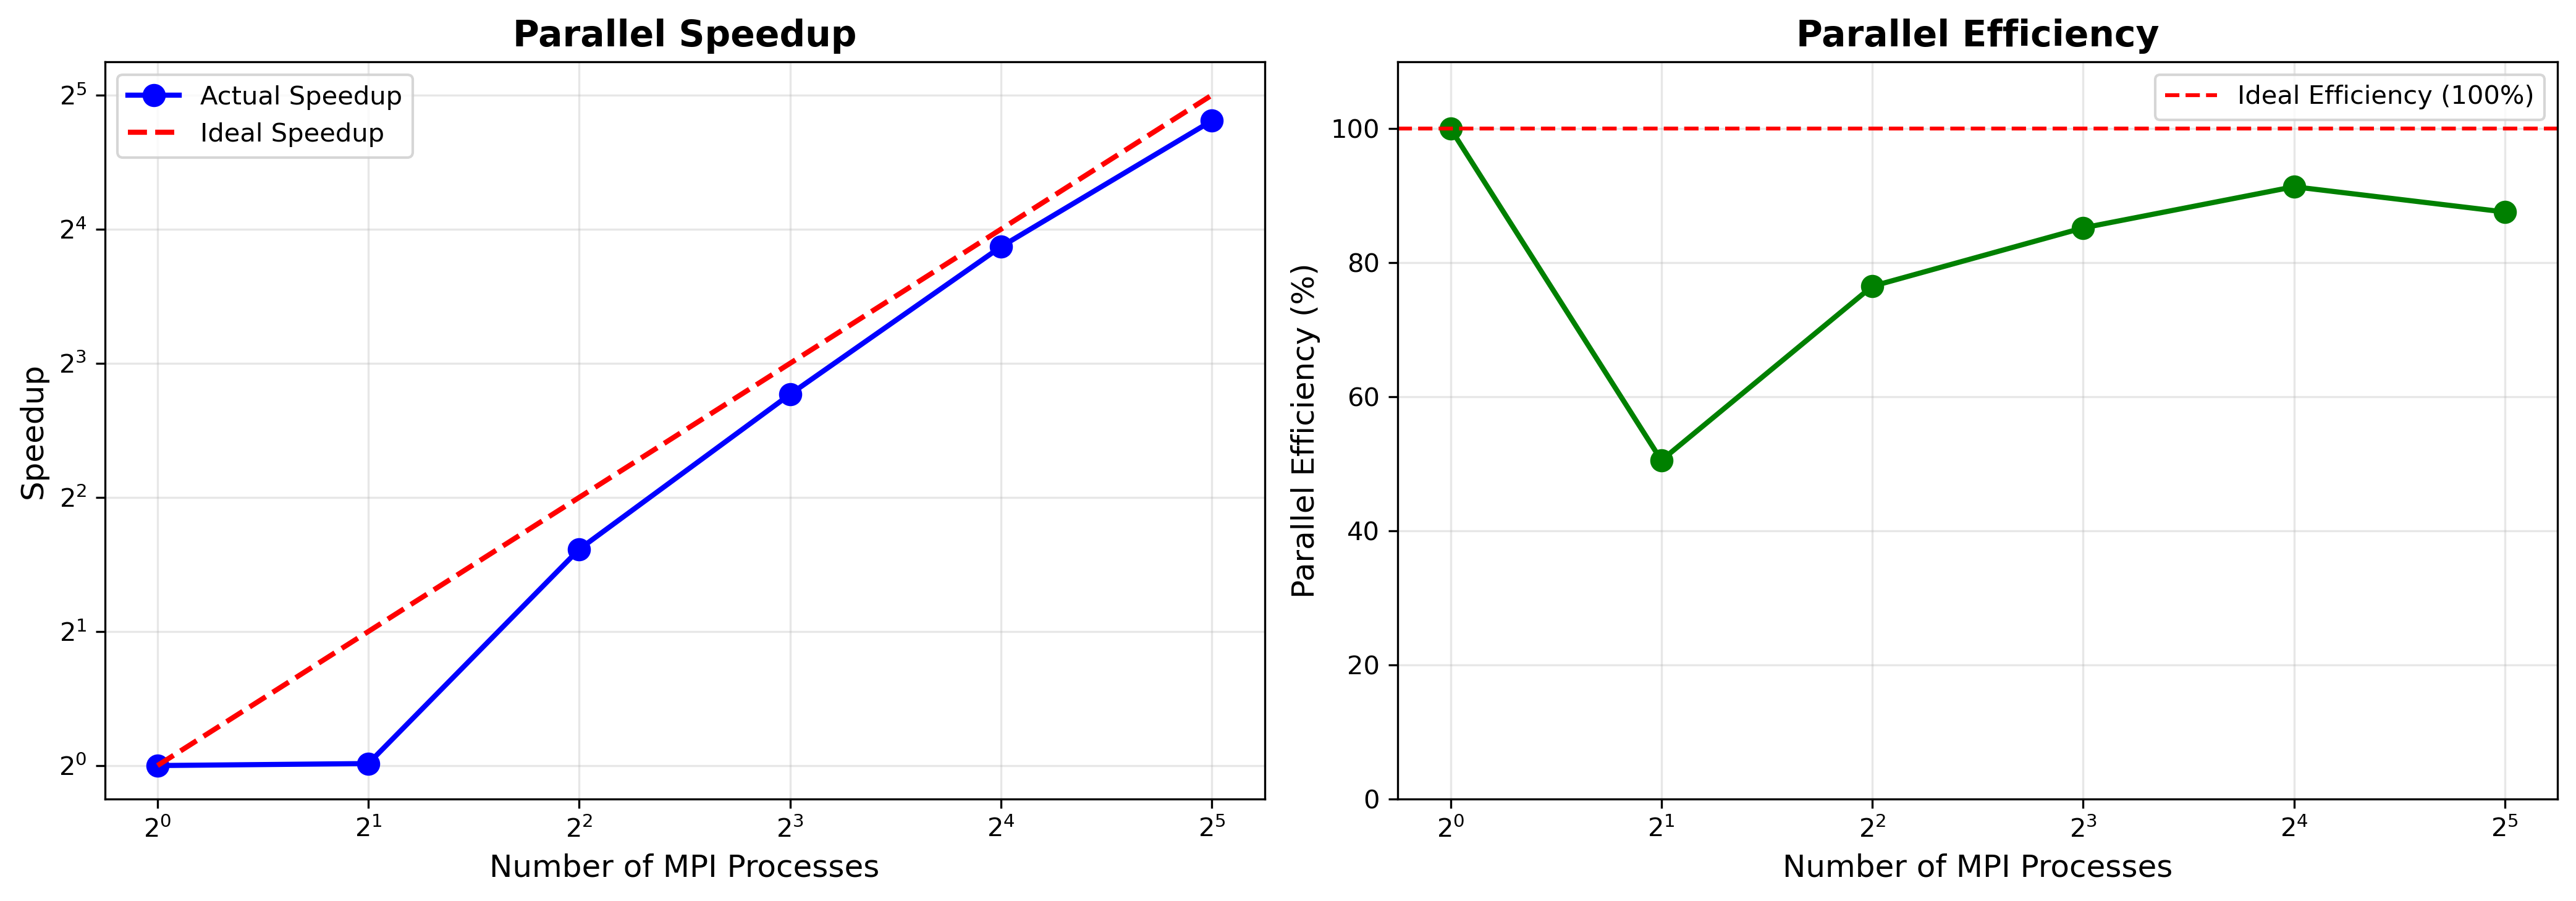
\includegraphics[width=\linewidth]{../scaling_plots.png}
		\caption{Strong scaling results: (left) Speedup vs. number of MPI processes showing actual performance compared to ideal linear speedup; (right) Parallel efficiency demonstrating sustained high performance up to 32 processes despite the anomalous 2-process case.}
		\label{fig:scaling}
	\end{figure}
	
	\section{Discussion}
	
	\subsection{Scaling Behavior}
	
	The results demonstrate \textbf{excellent strong scaling} from 4 to 32 processes:
	\begin{itemize}
		\item \textbf{4 processes}: Speedup of 3.06 (76.4\% efficiency)
		\item \textbf{8 processes}: Speedup of 6.81 (85.1\% efficiency)
		\item \textbf{16 processes}: Speedup of 14.61 (91.3\% efficiency)
		\item \textbf{32 processes}: Speedup of 28.04 (87.6\% efficiency)
	\end{itemize}
	
	The efficiency actually \textit{increases} from 4 to 16 processes before declining slightly at 32. This behavior suggests that:
	\begin{enumerate}
		\item The dynamic load balancing is working effectively
		\item Communication overhead remains minimal even at 32 processes
		\item Cache effects may play a role at lower process counts
	\end{enumerate}
	
	\subsection{The 2-Process Anomaly}
	
	The 2-process case shows virtually no speedup (1.01×, 50.5\% efficiency), which is unexpected. This can be explained by the master-worker architecture:
	\begin{itemize}
		\item With 2 processes: 1 master + 1 worker
		\item Master spends time managing work distribution and receiving results
		\item Only 1 worker performs actual computation
		\item Effectively similar to serial performance plus communication overhead
	\end{itemize}
	
	This confirms that the master-worker pattern requires $\geq 3$ processes to show benefits. With 4 processes (1 master + 3 workers), we achieve 3.06× speedup, close to the ideal 3× speedup for 3 computational workers.
	
	\subsection{Load Balancing Effectiveness}
	
	The Mandelbrot set exhibits highly variable computational cost per pixel:
	\begin{itemize}
		\item Pixels deep inside the set: exactly $n_{\text{max}}$ iterations
		\item Pixels far outside: very few iterations (fast escape)
		\item Pixels near the boundary: variable, often many iterations
	\end{itemize}
	
	Additionally, frames at different zoom levels have different overall costs. The dynamic master-worker approach successfully handles this heterogeneity, as evidenced by:
	\begin{itemize}
		\item Low standard deviation across runs (< 1 second in most cases)
		\item Sustained high efficiency even at 32 processes
		\item No evidence of idle workers or load imbalance
	\end{itemize}
	
	\subsection{Communication Overhead}
	
	The frame-level parallelization strategy minimizes communication:
	\begin{itemize}
		\item Each worker sends/receives only 2-3 small messages per frame
		\item No pixel data transfer when \texttt{store\_images=no}
		\item Total communication volume: $O(\text{frames})$, not $O(\text{pixels})$
	\end{itemize}
	
	This explains why parallel efficiency remains high (87.6\%) even at 32 processes.
	
	\subsection{Comparison to Alternative Approaches}
	
	Alternative parallelization strategies considered but not implemented:
	
	\textbf{Static frame distribution:} Assign frames 1-30 to process 0, 31-60 to process 1, etc.
	\begin{itemize}
		\item \textcolor{red}{Disadvantage}: Different frames have different costs; would cause load imbalance
		\item \textcolor{green}{Advantage}: No master overhead, simpler implementation
	\end{itemize}
	
	\textbf{Row-based parallelization:} Divide each frame into horizontal strips
	\begin{itemize}
		\item \textcolor{green}{Advantage}: Can parallelize a single frame
		\item \textcolor{red}{Disadvantage}: Much higher communication overhead
		\item \textcolor{red}{Disadvantage}: Complex I/O coordination for image writing
	\end{itemize}
	
	The chosen dynamic frame-level approach provides the best balance of simplicity, load balancing, and communication efficiency for this problem.
	
	\subsection{Bottlenecks and Limitations}
	
	\textbf{Identified bottlenecks:}
	\begin{enumerate}
		\item \textbf{Master process overhead}: At very high process counts (64+), the master may become a bottleneck managing many workers
		\item \textbf{Limited scalability beyond frames}: Cannot use more processes than frames (120 in our case)
		\item \textbf{I/O serialization}: When storing images, master must write sequentially
	\end{enumerate}
	
	\textbf{Amdahl's Law analysis:}
	The theoretical speedup is limited by the serial fraction $f_s$:
	\begin{equation}
		S(p) = \frac{1}{f_s + \frac{1-f_s}{p}}
	\end{equation}
	
	From our data at $p=32$: $S(32) = 28.04 \implies f_s \approx 0.012$ (1.2\% serial fraction).
	
	This very low serial fraction confirms the problem is highly parallelizable.
	
	\section{Conclusion}
	
	This assignment successfully demonstrated MPI parallelization of an embarrassingly parallel problem. Key achievements:
	\begin{itemize}
		\item Implemented efficient dynamic master-worker MPI parallelization
		\item Generated high-quality fractal visualizations including a Full HD zoom video
		\item Achieved 28.04× speedup on 32 processes (87.6\% efficiency)
		\item Demonstrated excellent load balancing and minimal communication overhead
		\item Confirmed embarrassingly parallel nature with only 1.2\% serial fraction
	\end{itemize}
	
	\textbf{Performance highlights:}
	\begin{itemize}
		\item Near-linear scaling from 4 to 32 processes
		\item Reduced computation time from 31 minutes (1 process) to 66 seconds (32 processes)
		\item High reproducibility (standard deviation < 1 second)
	\end{itemize}
	
	\textbf{Future improvements:}
	\begin{enumerate}
		\item \textbf{Hierarchical master-worker}: For 64+ processes, use multiple master processes
		\item \textbf{Hybrid approach}: Combine frame-level and row-level parallelization
		\item \textbf{Parallel I/O}: Use MPI-IO for concurrent image writing
		\item \textbf{Adaptive zoom}: Automatically detect interesting regions for deeper zoom
	\end{enumerate}
	
	The Mandelbrot set proved to be an excellent testbed for learning MPI programming, demonstrating how proper work distribution and minimal communication can achieve near-optimal parallel efficiency.
	
	\section*{Acknowledgments}
	
	I thank the Professors for providing the assignment framework and access to the Shabyt computing cluster. The assignment template and PPM writer code snippets were provided in the course materials. Claude 3.5 Sonnet assisted with code development, debugging, and report.
	
	\section*{Honor Statement}
	\honor
	
	\section*{Submission Checklist}
	\begin{itemize}
		\item[$\checkmark$] PDF report: \texttt{report\_a4\_akimshe.pdf}
		\item[$\checkmark$] Source code: \texttt{mandelbrot\_serial.cpp}, \texttt{mandelbrot\_mpi.cpp}
		\item[$\checkmark$] Build system: \texttt{Makefile}
		\item[$\checkmark$] Documentation: \texttt{README.md}
		\item[$\checkmark$] Video file: \texttt{video.mp4} (Full HD, 600 frames)
		\item[$\checkmark$] SLURM script: \texttt{run\_scaling.sh}
		\item[$\checkmark$] Analysis script: \texttt{analyze\_results.py}
		\item[$\checkmark$] High-resolution image: \texttt{mandelbrot\_full\_set.png}
	\end{itemize}
	
	\appendix
	\section{Complete Timing Data}
	
	Table~\ref{table:timings_detailed} presents the complete timing data from all individual runs.
	
	\begin{table}[H]
		\centering
		\caption{Detailed timing results (all individual runs).}
		\label{table:timings_detailed}
		\begin{tabular}{rrrrrr}
			\toprule
			Processes & Run 1 (s) & Run 2 (s) & Run 3 (s) & Mean (s) & Std Dev (s) \\
			\midrule
			1  & 1862.07 & 1863.93 & 1863.22 & 1863.07 & 0.94 \\
			2  & 1842.80 & 1842.51 & 1842.95 & 1842.75 & 0.23 \\
			4  & 608.60  & 610.29  & 609.48  & 609.46  & 0.85 \\
			8  & 273.19  & 273.55  & 273.89  & 273.54  & 0.35 \\
			16 & 127.42  & 127.52  & 127.61  & 127.51  & 0.09 \\
			32 & 66.45   & 66.40   & 66.50   & 66.45   & 0.05 \\
			\bottomrule
		\end{tabular}
	\end{table}
	
	\section{Source Code Organization}
	
	\textbf{File structure:}
	\begin{itemize}
		\item \texttt{mandelbrot\_serial.cpp} — Serial implementation (400 lines)
		\item \texttt{mandelbrot\_mpi.cpp} — MPI parallel implementation (450 lines)
		\item \texttt{Makefile} — Build configuration
		\item \texttt{README.md} — Build and run instructions
		\item \texttt{run\_scaling.sh} — SLURM batch script for scaling tests
		\item \texttt{analyze\_results.py} — Python script for data analysis and plotting
	\end{itemize}
	
	Both C++ implementations include:
	\begin{itemize}
		\item Mandelbrot iteration kernel
		\item Color mapping function
		\item PPM file writer
		\item Command-line argument parsing
		\item Frame generation with zoom progression
	\end{itemize}
	
	The MPI version adds:
	\begin{itemize}
		\item Master-worker communication using \texttt{MPI\_Send}/\texttt{MPI\_Recv}
		\item Dynamic work distribution logic
		\item Frame ordering and optional I/O handling
	\end{itemize}
	
\end{document}